\documentclass[tikz]{standalone}
\usepackage{tikz}
\usepackage{amssymb}
\usetikzlibrary{positioning}
\usetikzlibrary{calc}
\usetikzlibrary{arrows,shapes,snakes,automata,petri}
\begin{document}
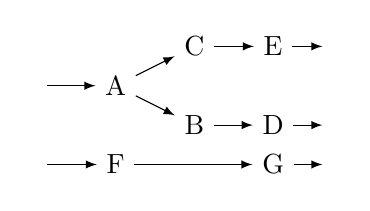
\begin{tikzpicture}
\node[](startA) at (-1,0){};
\node[](A) at (0,0){A};
\node[](B) at (1,-0.5){B};
\node[](C) at (1,0.5){C};
\node[](D) at (2,-0.5){D};
\node[](E) at (2,0.5){E};
\node[](endD) at (2.75,-0.5){};
\node[](endE) at (2.75,0.5){};
\node[](F) at (0,-1){F};
\node[](G) at (2,-1){G};

\node[](startF) at (-1,-1){};
\node[](endGA) at (2.75,-1){};

\path
(startA) edge[-latex]node{} (A)
(startF) edge[-latex]node{} (F)
(A) edge[-latex]node{} (B)
(A) edge[-latex]node{} (C)
(B) edge[-latex]node{} (D)
(C) edge[-latex]node{} (E)
(F) edge[-latex]node{} (G)
(E) edge[-latex]node{} (endE)
(G) edge[-latex]node{} (endGA)
(D) edge[-latex]node{} (endD);
\end{tikzpicture}
\end{document}